\documentclass[12pt]{standalone}
\usepackage{tikz}
\usetikzlibrary{arrows.meta, positioning}

\begin{document}
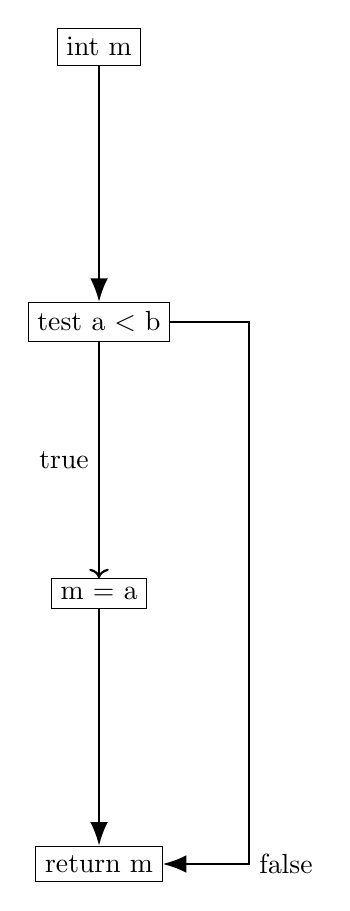
\begin{tikzpicture}[
    node distance=3cm and 4cm, 
    node/.style={draw, rectangle, text width=3cm, text centered, minimum height=1cm},
    arrow/.style={-{Latex[length=3mm]}, thick}
    ]

    \node[draw] (a_init) {int m};
    \node[draw, below=of a_init] (a_cond) {test a $<$ b};
    \node[draw, below=of a_cond] (a_true) {m = a};
    \node[draw, below=of a_true] (a_return) {return m};

    \draw[arrow] (a_init) -- (a_cond);
    \draw[thick, ->]  (a_cond) -- (a_true) node[midway, left] {true};
    \draw[arrow] (a_cond.east) -- ++(1,0) |- (a_return.east) node[midway, right] {false};
    \draw[arrow] (a_true) -- (a_return);

\end{tikzpicture}
\end{document}